%% bare_conf_compsoc.tex
%% V1.4b
%% 2015/08/26
%% by Michael Shell
%% See:
%% http://www.michaelshell.org/
%% for current contact information.
%%
%% This is a skeleton file demonstrating the use of IEEEtran.cls
%% (requires IEEEtran.cls version 1.8b or later) with an IEEE Computer
%% Society conference paper.
%%
%% Support sites:
%% http://www.michaelshell.org/tex/ieeetran/
%% http://www.ctan.org/pkg/ieeetran
%% and
%% http://www.ieee.org/

\documentclass[conference,compsoc]{IEEEtran}
% Some/most Computer Society conferences require the compsoc mode option,
% but others may want the standard conference format.
%
% If IEEEtran.cls has not been installed into the LaTeX system files,
% manually specify the path to it like:
% \documentclass[conference,compsoc]{../sty/IEEEtran}

% *** MISC UTILITY PACKAGES ***
%
\usepackage{ifpdf}
\usepackage{framed}
% Heiko Oberdiek's ifpdf.sty is very useful if you need conditional
% compilation based on whether the output is pdf or dvi.
% usage:
% \ifpdf
%   % pdf code
% \else
%   % dvi code
% \fi
% The latest version of ifpdf.sty can be obtained from:
% http://www.ctan.org/pkg/ifpdf
% Also, note that IEEEtran.cls V1.7 and later provides a builtin
% \ifCLASSINFOpdf conditional that works the same way.
% When switching from latex to pdflatex and vice-versa, the compiler may
% have to be run twice to clear warning/error messages.



% *** CITATION PACKAGES ***
%
\ifCLASSOPTIONcompsoc
  % IEEE Computer Society needs nocompress option
  % requires cite.sty v4.0 or later (November 2003)
  \usepackage[nocompress]{cite}
\else
  % normal IEEE
  \usepackage{cite}
\fi
% cite.sty was written by Donald Arseneau
% V1.6 and later of IEEEtran pre-defines the format of the cite.sty package
% \cite{} output to follow that of the IEEE. Loading the cite package will
% result in citation numbers being automatically sorted and properly
% "compressed/ranged". e.g., [1], [9], [2], [7], [5], [6] without using
% cite.sty will become [1], [2], [5]--[7], [9] using cite.sty. cite.sty's
% \cite will automatically add leading space, if needed. Use cite.sty's
% noadjust option (cite.sty V3.8 and later) if you want to turn this off
% such as if a citation ever needs to be enclosed in parenthesis.
% cite.sty is already installed on most LaTeX systems. Be sure and use
% version 5.0 (2009-03-20) and later if using hyperref.sty.
% The latest version can be obtained at:
% http://www.ctan.org/pkg/cite
% The documentation is contained in the cite.sty file itself.
%
% Note that some packages require special options to format as the Computer
% Society requires. In particular, Computer Society  papers do not use
% compressed citation ranges as is done in typical IEEE papers
% (e.g., [1]-[4]). Instead, they list every citation separately in order
% (e.g., [1], [2], [3], [4]). To get the latter we need to load the cite
% package with the nocompress option which is supported by cite.sty v4.0
% and later.





% *** GRAPHICS RELATED PACKAGES ***
%
\ifCLASSINFOpdf
  % \usepackage[pdftex]{graphicx}
  % declare the path(s) where your graphic files are
  % \graphicspath{{../pdf/}{../jpeg/}}
  % and their extensions so you won't have to specify these with
  % every instance of \includegraphics
  % \DeclareGraphicsExtensions{.pdf,.jpeg,.png}
\else
  % or other class option (dvipsone, dvipdf, if not using dvips). graphicx
  % will default to the driver specified in the system graphics.cfg if no
  % driver is specified.
  % \usepackage[dvips]{graphicx}
  % declare the path(s) where your graphic files are
  % \graphicspath{{../eps/}}
  % and their extensions so you won't have to specify these with
  % every instance of \includegraphics
  % \DeclareGraphicsExtensions{.eps}
\fi
% graphicx was written by David Carlisle and Sebastian Rahtz. It is
% required if you want graphics, photos, etc. graphicx.sty is already
% installed on most LaTeX systems. The latest version and documentation
% can be obtained at: 
% http://www.ctan.org/pkg/graphicx
% Another good source of documentation is "Using Imported Graphics in
% LaTeX2e" by Keith Reckdahl which can be found at:
% http://www.ctan.org/pkg/epslatex
%
% latex, and pdflatex in dvi mode, support graphics in encapsulated
% postscript (.eps) format. pdflatex in pdf mode supports graphics
% in .pdf, .jpeg, .png and .mps (metapost) formats. Users should ensure
% that all non-photo figures use a vector format (.eps, .pdf, .mps) and
% not a bitmapped formats (.jpeg, .png). The IEEE frowns on bitmapped formats
% which can result in "jaggedy"/blurry rendering of lines and letters as
% well as large increases in file sizes.
%
% You can find documentation about the pdfTeX application at:
% http://www.tug.org/applications/pdftex





% *** MATH PACKAGES ***
%
\usepackage{amsmath}
\usepackage{cuted}
% A popular package from the American Mathematical Society that provides
% many useful and powerful commands for dealing with mathematics.
%
% Note that the amsmath package sets \interdisplaylinepenalty to 10000
% thus preventing page breaks from occurring within multiline equations. Use:
%\interdisplaylinepenalty=2500
% after loading amsmath to restore such page breaks as IEEEtran.cls normally
% does. amsmath.sty is already installed on most LaTeX systems. The latest
% version and documentation can be obtained at:
% http://www.ctan.org/pkg/amsmath
\newcommand\numberthis{\addtocounter{equation}{1}\tag{\theequation}}




% *** SPECIALIZED LIST PACKAGES ***
%
\usepackage{algorithmic}
% algorithmic.sty was written by Peter Williams and Rogerio Brito.
% This package provides an algorithmic environment fo describing algorithms.
% You can use the algorithmic environment in-text or within a figure
% environment to provide for a floating algorithm. Do NOT use the algorithm
% floating environment provided by algorithm.sty (by the same authors) or
% algorithm2e.sty (by Christophe Fiorio) as the IEEE does not use dedicated
% algorithm float types and packages that provide these will not provide
% correct IEEE style captions. The latest version and documentation of
% algorithmic.sty can be obtained at:
% http://www.ctan.org/pkg/algorithms
% Also of interest may be the (relatively newer and more customizable)
% algorithmicx.sty package by Szasz Janos:
% http://www.ctan.org/pkg/algorithmicx




% *** ALIGNMENT PACKAGES ***
%
\usepackage{array}
% Frank Mittelbach's and David Carlisle's array.sty patches and improves
% the standard LaTeX2e array and tabular environments to provide better
% appearance and additional user controls. As the default LaTeX2e table
% generation code is lacking to the point of almost being broken with
% respect to the quality of the end results, all users are strongly
% advised to use an enhanced (at the very least that provided by array.sty)
% set of table tools. array.sty is already installed on most systems. The
% latest version and documentation can be obtained at:
% http://www.ctan.org/pkg/array


% IEEEtran contains the IEEEeqnarray family of commands that can be used to
% generate multiline equations as well as matrices, tables, etc., of high
% quality.




% *** SUBFIGURE PACKAGES ***
%\ifCLASSOPTIONcompsoc
%  \usepackage[caption=false,font=footnotesize,labelfont=sf,textfont=sf]{subfig}
%\else
%  \usepackage[caption=false,font=footnotesize]{subfig}
%\fi
% subfig.sty, written by Steven Douglas Cochran, is the modern replacement
% for subfigure.sty, the latter of which is no longer maintained and is
% incompatible with some LaTeX packages including fixltx2e. However,
% subfig.sty requires and automatically loads Axel Sommerfeldt's caption.sty
% which will override IEEEtran.cls' handling of captions and this will result
% in non-IEEE style figure/table captions. To prevent this problem, be sure
% and invoke subfig.sty's "caption=false" package option (available since
% subfig.sty version 1.3, 2005/06/28) as this is will preserve IEEEtran.cls
% handling of captions.
% Note that the Computer Society format requires a sans serif font rather
% than the serif font used in traditional IEEE formatting and thus the need
% to invoke different subfig.sty package options depending on whether
% compsoc mode has been enabled.
%
% The latest version and documentation of subfig.sty can be obtained at:
% http://www.ctan.org/pkg/subfig
\usepackage{verbatim}
\usepackage{soul}
\usepackage{xcolor}
\newcommand{\TODO}[1]{\hl{TODO: #1}}
\newcommand{\NOTE}[1]{\hl {NOTE: #1}}
\newcommand{\changed}[1]{\textcolor{red}{#1}}


% *** FLOAT PACKAGES ***
%
%\usepackage{fixltx2e}
% fixltx2e, the successor to the earlier fix2col.sty, was written by
% Frank Mittelbach and David Carlisle. This package corrects a few problems
% in the LaTeX2e kernel, the most notable of which is that in current
% LaTeX2e releases, the ordering of single and double column floats is not
% guaranteed to be preserved. Thus, an unpatched LaTeX2e can allow a
% single column figure to be placed prior to an earlier double column
% figure.
% Be aware that LaTeX2e kernels dated 2015 and later have fixltx2e.sty's
% corrections already built into the system in which case a warning will
% be issued if an attempt is made to load fixltx2e.sty as it is no longer
% needed.
% The latest version and documentation can be found at:
% http://www.ctan.org/pkg/fixltx2e


%\usepackage{stfloats}
% stfloats.sty was written by Sigitas Tolusis. This package gives LaTeX2e
% the ability to do double column floats at the bottom of the page as well
% as the top. (e.g., "\begin{figure*}[!b]" is not normally possible in
% LaTeX2e). It also provides a command:
%\fnbelowfloat
% to enable the placement of footnotes below bottom floats (the standard
% LaTeX2e kernel puts them above bottom floats). This is an invasive package
% which rewrites many portions of the LaTeX2e float routines. It may not work
% with other packages that modify the LaTeX2e float routines. The latest
% version and documentation can be obtained at:
% http://www.ctan.org/pkg/stfloats
% Do not use the stfloats baselinefloat ability as the IEEE does not allow
% \baselineskip to stretch. Authors submitting work to the IEEE should note
% that the IEEE rarely uses double column equations and that authors should try
% to avoid such use. Do not be tempted to use the cuted.sty or midfloat.sty
% packages (also by Sigitas Tolusis) as the IEEE does not format its papers in
% such ways.
% Do not attempt to use stfloats with fixltx2e as they are incompatible.
% Instead, use Morten Hogholm'a dblfloatfix which combines the features
% of both fixltx2e and stfloats:
%
% \usepackage{dblfloatfix}
% The latest version can be found at:
% http://www.ctan.org/pkg/dblfloatfix




% *** PDF, URL AND HYPERLINK PACKAGES ***
%
\usepackage{url}
% url.sty was written by Donald Arseneau. It provides better support for
% handling and breaking URLs. url.sty is already installed on most LaTeX
% systems. The latest version and documentation can be obtained at:
% http://www.ctan.org/pkg/url
% Basically, \url{my_url_here}.

\usepackage{graphicx} % Required for including pictures
\graphicspath{{pics/}} % Specifies the directory where pictures are stored
\usepackage{caption}
\usepackage{subcaption}



% *** Do not adjust lengths that control margins, column widths, etc. ***
% *** Do not use packages that alter fonts (such as pslatex).         ***
% There should be no need to do such things with IEEEtran.cls V1.6 and later.
% (Unless specifically asked to do so by the journal or conference you plan
% to submit to, of course. )


% correct bad hyphenation here
\hyphenation{op-tical net-works semi-conduc-tor}


\begin{document}
%
% paper title
% Titles are generally capitalized except for words such as a, an, and, as,
% at, but, by, for, in, nor, of, on, or, the, to and up, which are usually
% not capitalized unless they are the first or last word of the title.
% Linebreaks \\ can be used within to get better formatting as desired.
% Do not put math or special symbols in the title.
\title{Watch Out for the Bully! Study of Interference Between Jobs Running Concurrently on Dragonfly Network}


% author names and affiliations
% use a multiple column layout for up to three different
% affiliations
% \author{\IEEEauthorblockN{Michael Shell}
% \IEEEauthorblockA{School of Electrical and\\Computer Engineering\\
% Georgia Institute of Technology\\
% Atlanta, Georgia 30332--0250\\
% Email: http://www.michaelshell.org/contact.html}
% \and
% \IEEEauthorblockN{Homer Simpson}
% \IEEEauthorblockA{Twentieth Century Fox\\
% Springfield, USA\\
% Email: homer@thesimpsons.com}
% \and
% \IEEEauthorblockN{James Kirk\\ and Montgomery Scott}
% \IEEEauthorblockA{Starfleet Academy\\
% San Francisco, California 96678-2391\\
% Telephone: (800) 555--1212\\
% Fax: (888) 555--1212}}


\author{

\IEEEauthorblockN{Xu Yang\IEEEauthorrefmark{1}, John Jenkins\IEEEauthorrefmark{2}, Misbah Mubarak\IEEEauthorrefmark{2}, Robert B. Ross\IEEEauthorrefmark{2}, Zhiling Lan\IEEEauthorrefmark{1}}

\IEEEauthorblockA{\IEEEauthorrefmark{1}Department of Computer Science,
Illinois Institute of Technology,
Chicago, Illinois, USA 60616\\
\{xyang56\}@hawk.iit.edu, lan@iit.edu}

\IEEEauthorblockA{\IEEEauthorrefmark{2}Mathematics and Computer Science Division, Argonne National Laboratory,
Argonne, IL, USA 60439\\
\{jenkins,rross\}@mcs.anl.gov, mmubarak@anl.gov}
}


% conference papers do not typically use \thanks and this command
% is locked out in conference mode. If really needed, such as for
% the acknowledgment of grants, issue a \IEEEoverridecommandlockouts
% after \documentclass

% for over three affiliations, or if they all won't fit within the width
% of the page (and note that there is less available width in this regard for
% compsoc conferences compared to traditional conferences), use this
% alternative format:
% 
%\author{\IEEEauthorblockN{Michael Shell\IEEEauthorrefmark{1},
%Homer Simpson\IEEEauthorrefmark{2},
%James Kirk\IEEEauthorrefmark{3}, 
%Montgomery Scott\IEEEauthorrefmark{3} and
%Eldon Tyrell\IEEEauthorrefmark{4}}
%\IEEEauthorblockA{\IEEEauthorrefmark{1}School of Electrical and Computer Engineering\\
%Georgia Institute of Technology,
%Atlanta, Georgia 30332--0250\\ Email: see http://www.michaelshell.org/contact.html}
%\IEEEauthorblockA{\IEEEauthorrefmark{2}Twentieth Century Fox, Springfield, USA\\
%Email: homer@thesimpsons.com}
%\IEEEauthorblockA{\IEEEauthorrefmark{3}Starfleet Academy, San Francisco, California 96678-2391\\
%Telephone: (800) 555--1212, Fax: (888) 555--1212}
%\IEEEauthorblockA{\IEEEauthorrefmark{4}Tyrell Inc., 123 Replicant Street, Los Angeles, California 90210--4321}}




% use for special paper notices
%\IEEEspecialpapernotice{(Invited Paper)}




% make the title area
\maketitle

% As a general rule, do not put math, special symbols or citations
% in the abstract
\begin{abstract}

The high-radix, low-diameter dragonfly topology network will be the choice of many computing facilities for building their next generation supercomputers. Preliminary study shows that random job allocation with adaptive routing would be the rule of thumb to utilize such powerful network. However, in this work, we made the observation that although random job allocation with adaptive routing can alleviate the hotspot and make network traffic load-balanced for the workload, it can not guarantee the best performance for each single job. The performance improvement of communication intensive jobs comes with sacrifice of those less intensive jobs. We refer this phenomenon as ``bully" between concurrently running jobs. In this paper, we analyze the detailed reason for the happening of this ``bully" from the network level. Our study is based on a sophisticated, high-fidelity discrete even-driven simulation tool. We believe the observations and analysis in this work will make the chosen of job allocation and routing strategies more cautiously in future.


\end{abstract}

% no keywords




% For peer review papers, you can put extra information on the cover
% page as needed:
% \ifCLASSOPTIONpeerreview
% \begin{center} \bfseries EDICS Category: 3-BBND \end{center}
% \fi
%
% For peerreview papers, this IEEEtran command inserts a page break and
% creates the second title. It will be ignored for other modes.
\IEEEpeerreviewmaketitle



\section{Introduction}
\label{sec:intro}

The dragonfly topology can provide the ability for building high-radix, low-diameter network that are preferable for HPC systems. Compared with Torus topology, dragonfly can provide high-bandwidth, low-latency that are attractive for building multi-Petaflop/s supercomputers\cite{dally-dragonfly}. The procurement results from Trinity and CORAL project shows the great performance improvement from dragonfly network. 


Even with such powerful network, the interference between concurrently running jobs is still a major factor impacting jobs' performance \cite{bhatele2015, dskinner}. Some research work propose that random job placement coupled with adaptive routing strategies can alleviate local congestion, eliminate hot-spots and reach load-balance for dragonfly networks \cite{jain-sc14, bhatele-sc11, brandt2014}. They got this conclusion with different simulation tools and various synthetic workloads.

This is paper, we study the interference between concurrently running jobs on Dragonfly network with different job allocation policies and routing algorithms. Being unorthodox to most existing work, we use real application traces that collected from production system instead of synthetic workloads. The advantage of using real application traces is quite obvious. The traces collected from production system can capture application's communication behavior in detail that usually omitted in synthetic workload for the purpose of simplicity. 


We also evaluate the network performance and jobs' performance when the Dragonfly network is configured with different job allocation strategies and routing algorithms. The job allocation strategies used in our study are Compact allocation and Random allocation, both of which can be seen in existing production HPC systems. The routing strategies been analyzed in this work are Minimal, Nonminimal and Adaptive.  


We made observation from our comprehensive study that, when dragonfly network enabled with random job allocation and adaptive routing in order to reach hot-spot free and load balance, the performance of particular job would be impaired. The communication intensive jobs in the workload can benefit from random allocation and adaptive routing, with great performance improvement. Unfortunately, those less intensive jobs are the sacrifices for this improvement, their performance will be greatly reduced. The findings in this work also reconfirm that interference between concurrently running jobs would make the performance of some jobs every unpredictable. The detailed analysis about the traffic and congestion in network level unveil the undercurrent beneath that interference.  

This work makes the following contributions:

\begin{itemize}
   
    \item Our real trace-based analysis about job interference on dragonfly network, shows that random allocation with adaptive routing can not guarantee the performance of every job in the workload. The hotspot-free and load-balanced reached by using random allocation with adaptive routing come with the cost of communication-less-intensive jobs performance degradation. 

    \item We identify the ``bully" happening between jobs running concurrently on dragonfly network with random allocation and adaptive routing. Random allocation and adaptive routing redirect the traffic of communication intensive jobs to the routers through which less intensive jobs' traffic used to go, embezzle the network resources(such as router ports and links), slow down the communication of those less intensive jobs.

    
    \item We found that compact allocation and minimal routing can guarantee the consistent performance of each job running on dragonfly network, while may leads to local hotspot and severe network congestion. Actually, compact allocation and minimal routing are preferred by communication-less-intensive jobs, since it will prevent them from being bullied by other communication-intensive jobs.
    
         
\end{itemize}

To the best of our knowledge, using real application traces for the study of job interference on dragonfly network as not been reported so far. We believe the observations and analysis presented in this paper can be used by computing facilities to choose  job allocation and routing strategies wisely for their future dragonfly interconnected system. The conclusion from this paper would be useful for batch schedulers in dragonfly system to make better scheduling decisions for jobs with specific communication behavior.


\section{Dragonfly Network}
\label{sec:network}
It is difficult to do experiment with concurrently running jobs on HPC system. One reason is that job placement and routing strategy are part of system configuration, it is impossible for user to make changes at will. Another reason is that it is unrealistic to reserve the system exclusively to run the same batch of jobs with desired placement and routing configurations and compare the results. Therefore, we resort to simulation in our work.

A simulation toolkit named CODES enables the exploration of simulating different HPC networks with high fidelity and great scalability\cite{codes}.  CODES support dragonfly network with high fidelity flit-level simulation\cite{codes-dragonfly}. It has this network workload component that is capable of taking real MPI application traces generated by SST DUMPI\cite{sst} for trace-driven simulations.

\subsection{Network Configuration}
\label{sec: network config}
 
Here will talk about network configuration, such as network scale, link bandwidth etc.\\


\subsection{Job Placement}
\label{sec:placement-routing}

Job placement refers to the scheme used by batch scheduler to allocate the required number of nodes by the job for execution. There are many works study various ways of doing job placement on HPC systems with different topologies \cite{yang-cluster14} \cite{zhou-ipdps15} \cite{hoefler-hpdc14}. In this work, we study the following two placement schemes:

\textbf{Contiguous Placement:} In this scheme, the nodes will first be indexed consecutively in the increasing oder of their group id and router id. The job is allocated by cutting chunks of nodes from the sequentially ordered list. The nodes been allocated to each job will be adjacent to each other, usually they are attached to the same router, in the same group. Contiguous placement confines the traffic of application into the local area, which may leads to local network congestion and increase the possibility of hot-spots. 

\textbf{Random Placement:} In this scheme, job will get a set of nodes that randomly selected from all the available nodes in the system. The nodes allocated to each job would be attached to different routers in different groups. Some routers may be shared by different applications when using random placement. Random placement can spreading the traffic of application uniformly across the whole system, thus avoid the possible hot-spots and reach load balance.


\subsection{Routing Schemes}
\label{sec:routing}

The implemented routing schemes in CODES dragonfly network model are based on the routing algorithm proposed by Kim et al. \cite{dally-dragonfly}. Two routing schemes studied in this work are \emph{Minimal} and \emph{Adaptive}.

\textbf{Minimal:} The minimal routing sends a message from source router to destination router along the shortest path. When there are multiple shortest paths, the message is evenly divided among the paths. Minimal routing can guarantee the minimum hops the message takes from source to destination. However, it may leads to congestion along the shortest path. 


\textbf{Adaptive:} In this scheme, the path a message takes will be adaptively chosen between shortest and non-shortest path, depends on the congestion situation along that path. For the non-shortest path, an intermediate router will be randomly chosen. The message will first take the shortest path from source to that intermediate router, then it will take the shortest path between the intermediate router to the destination. Since adaptive scheme chooses routing path adaptively based on the congestion situation, it can void local congestion and reduce the possibility of hot-spots. 


\section{Evaluation}
\label{sec:evaluation}

\subsection{Application}
\label{sec:app study}

We choose three representative applications from DOE Design Forward Project\cite{designforwardwebpage}. . We believe these applications can be representative of a wide array of applications running on leadership-class supercomputers. Specifically, we study the Algebraic MultiGrid Solver (AMG), Geometric MultiGrid (MultiGrid) and CrystalRouter MiniApps. 

AMG: The Algebraic MultiGrid Solver, is a parallel algebraic multi-grid solver for linear systems arising from problems on unstructured mesh physics packages. It has been derived directly from the BoomerAMG solver that is being developed in the Center for Applied Scientific Computing (CASC) at LLNL\cite{amg}.

MultiGrid: massively parallel block-structured adaptive mesh refinement (AMR) codes a software framework for massively parallel block-structured adaptive mesh refinement (AMR) codes\cite{boxlib}. It is widely used for structured grid physics packages.

CrystalRouter: the extracted communication kernel of the full application Nek5000\cite{nek5000}, which is a spectral element CFD application developed at Argonne National Laboratory\cite{crystalrouter}. It features spectral element multi-grid solvers coupled with a highly scalable, parallel coarse-grid solver that is widely used for projects including ocean current modeling, thermal hydraulics of reactor cores,and spatiotemporal chaos.


\subsection{Workload Overview}
\label{sec: workload overview}

We make a workload that consists of these three applications and simulate the running of this workload on dragonfly network. In our simulation, we adopt two job placement policies, Contiguous and Random, for mapping application MPI ranks to network terminal nodes. We also try two routing algorithms are commonly used in dragonfly network, Adaptive and Minimal. Therefore, there are 4 configurations “Contiguous placement with Adaptive routing” , “Contiguous placement with Minimal routing”, “Random placement with  Adaptive routing” and “Random placement with Minimal routing”. 


\begin{figure*}[t!]
    \centering
    \begin{subfigure}[t]{0.32\textwidth}
        \centering
        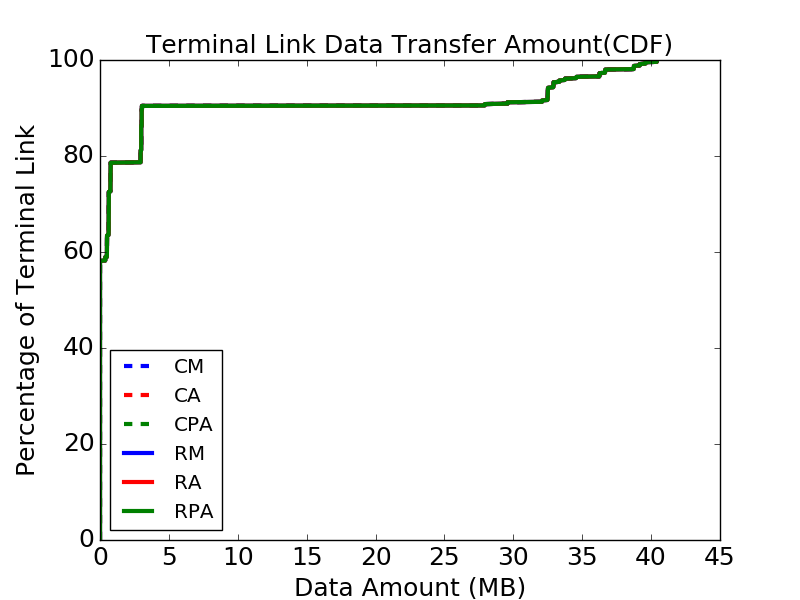
\includegraphics[height=1.8 in]{wkld/tl-traffic}
        \caption{Terminal Link Traffic}
        \label{fig:terminal-link-traffic}
    \end{subfigure}%
    \hspace{1em}%
    \begin{subfigure}[t]{0.32\textwidth}
        \centering
        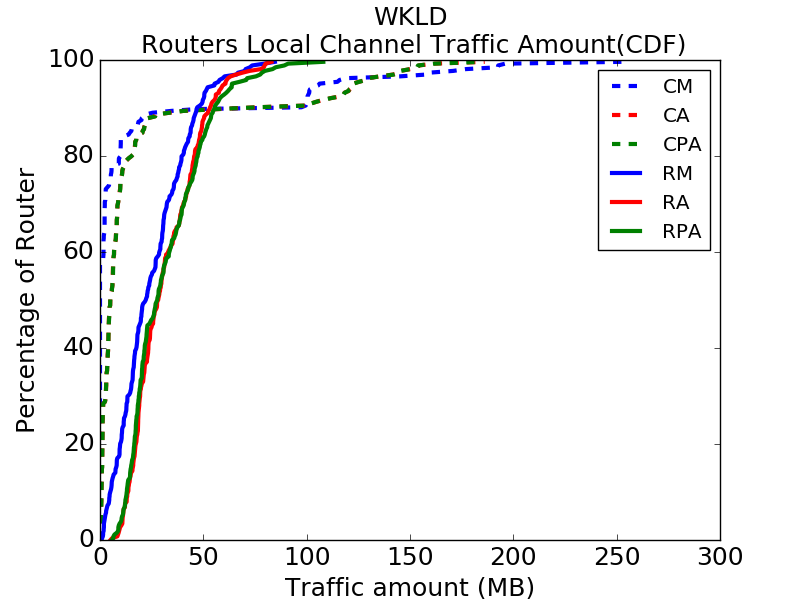
\includegraphics[height=1.8 in]{wkld/lc-traffic}
        \caption{Local Channel Traffic}
        \label{fig:local-channel-traffic}
    \end{subfigure}%
    \begin{subfigure}[t]{0.32\textwidth}
        \centering
        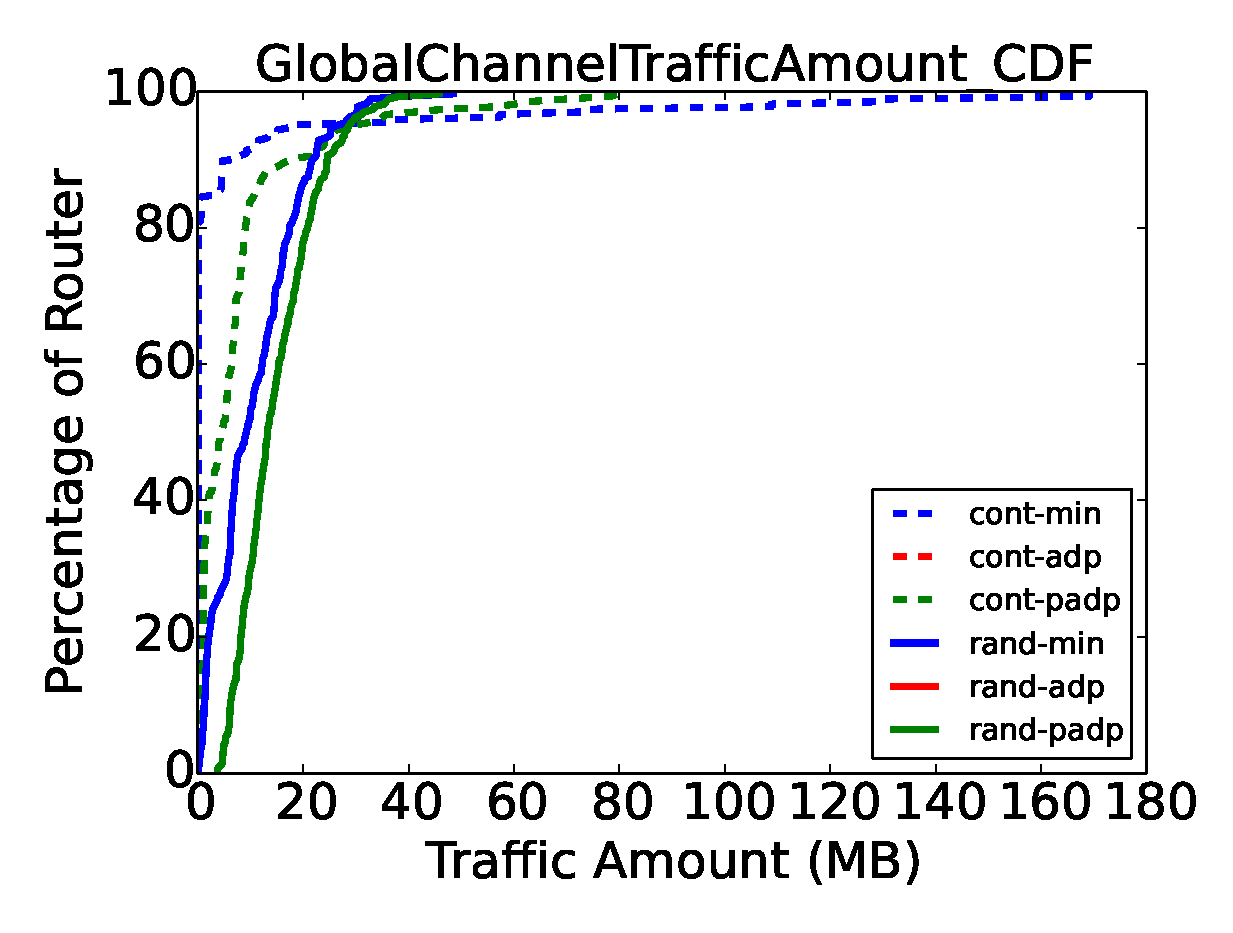
\includegraphics[height=1.8 in]{wkld/gc-traffic}
        \caption{Global Channel Traffic}
        \label{fig:global-channel-traffic}
    \end{subfigure}%
   \caption{Network Traffic. \textbf{More explanation to be added for this figure}}
   \label{fig:wkld-network-traffic}
\end{figure*}


\begin{figure*}[t!]
    \centering
    \begin{subfigure}[t]{0.32\textwidth}
        \centering
        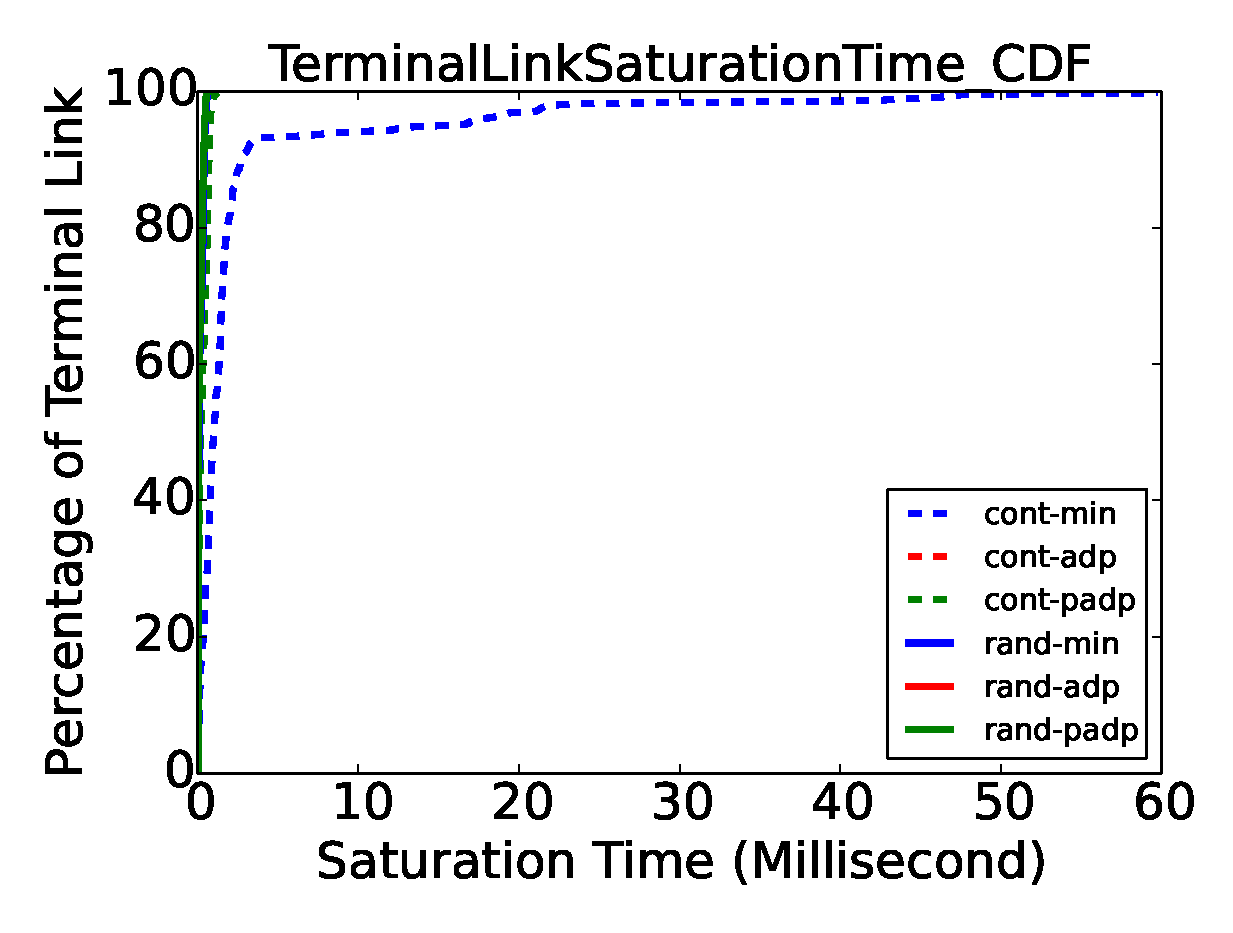
\includegraphics[height=1.8 in]{wkld/tl-stime}
        \caption{Terminal Link Busy Time}
        \label{fig:terminal-link-stime}
    \end{subfigure}%
    \hspace{1em}%
    \begin{subfigure}[t]{0.32\textwidth}
        \centering
        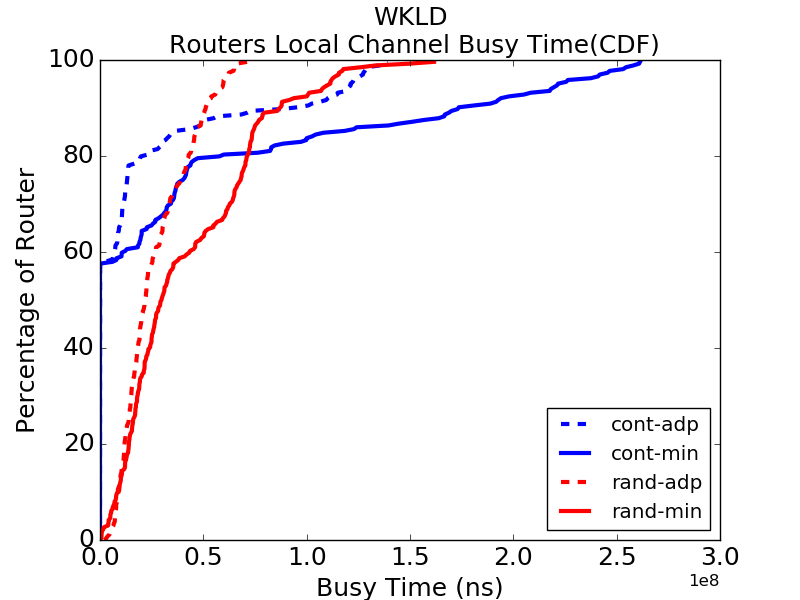
\includegraphics[height=1.8 in]{wkld/lc-stime}
        \caption{Local Channel Busy Time}
        \label{fig:local-channel-stime}
    \end{subfigure}%
    \begin{subfigure}[t]{0.32\textwidth}
        \centering
        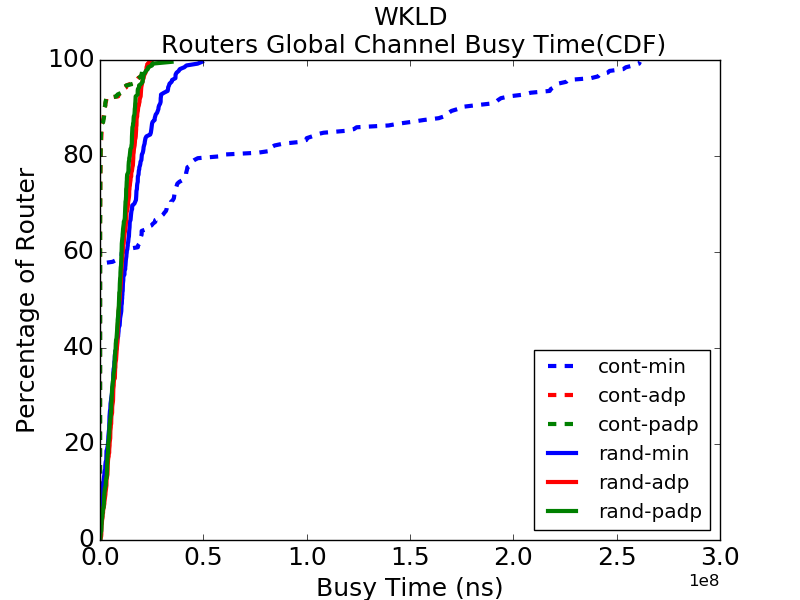
\includegraphics[height=1.8 in]{wkld/gc-stime}
        \caption{Global Channel Busy Time}
        \label{fig:global-channel-stime}
    \end{subfigure}%
   \caption{Network Channel Busy Time. \textbf{More explanation to be added for this figure}}
   \label{fig:wkld-network-stime}
\end{figure*}

Contiguous placement allocates each job a set of nodes that adjacent to each other, which confines the traffic of the application into the local area when coupled with minimal routing. This may leads to hot-spot in local area and unbalanced network utilization. As we can see from Figure \ref{fig:wkld-network-traffic} and \ref{fig:wkld-network-stime}, contiguous placement coupled with minimal routing always leads to the extreme high traffic amount for some routers , and thus longest network busytime.

Figure \ref{fig:wkld-network-traffic} and Figure \ref{fig:wkld-network-stime} shows that random job placement with adaptive routing can uniformly distribute workload traffic and balance the load over the network. 

\subsection{Application Analysis}
\label{sec:app analysis}

The random job placement and adaptive routing can reach hot-spots free and load-balanced by distributing the workload traffic over the network. In this section, we will show that not every application can benefit from random job placement and adaptive routing. 

\begin{figure*}[t!]
    \centering
    \begin{subfigure}[t]{0.32\textwidth}
        \centering
        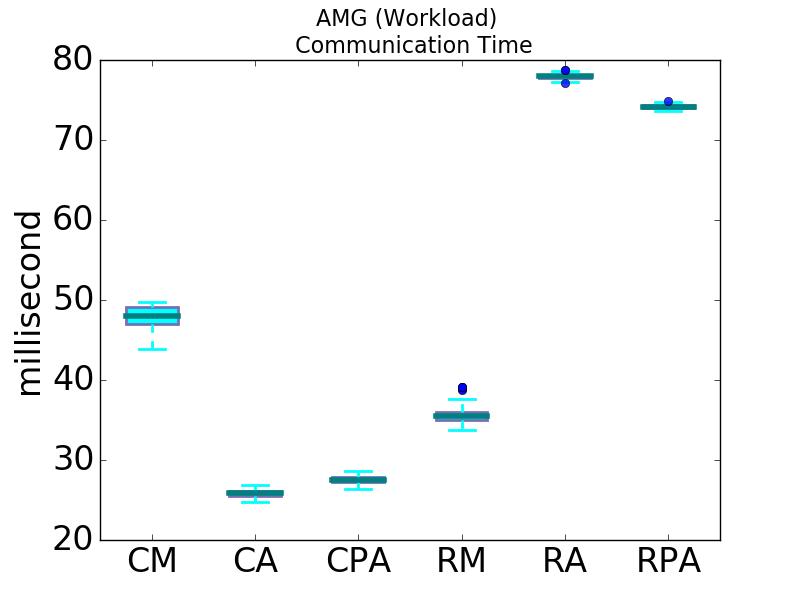
\includegraphics[height=1.5 in]{amg/commtime}
        \caption{AMG Communication Time}
        \label{fig:amg-commtime}
    \end{subfigure}%
    \hspace{1em}%
    \begin{subfigure}[t]{0.32\textwidth}
        \centering
        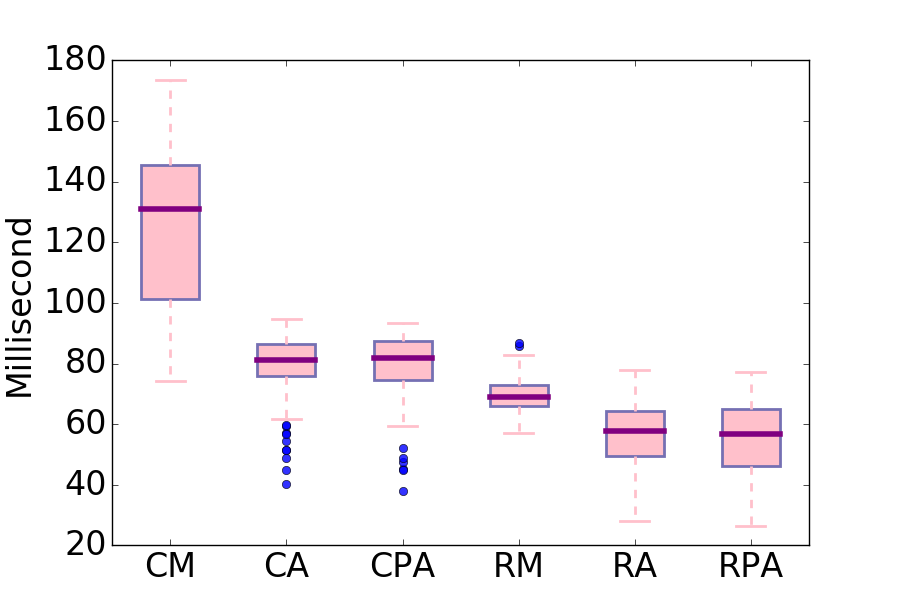
\includegraphics[height=1.5 in]{mg/commtime}
        \caption{MG Communication Time}
        \label{fig:mg-commtime}
    \end{subfigure}%
    \begin{subfigure}[t]{0.32\textwidth}
        \centering
        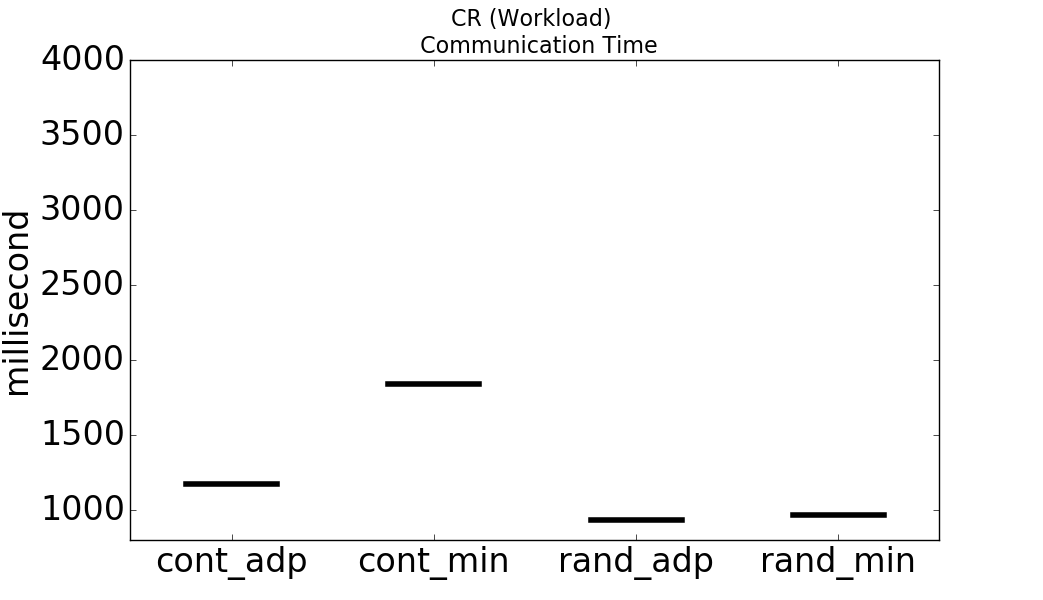
\includegraphics[height=1.5 in]{cr/commtime}
        \caption{CR Communication Time}
        \label{fig:cr-commtime}
    \end{subfigure}%
   \caption{Application communication time. Three applications running concurrently on dragonfly network with different placement and routing configurations. Random job placement and adaptive routing can improve MG and CR communication, however, AMG's communication time is greatly prolonged.}
   \label{fig:apps-commtime}
\end{figure*}

Figure \ref{fig:apps-commtime} shows the communication time of three applications running concurrently with 4 different placement and routing configurations. MG and CR can get improvement with random placement and adaptive routing, compared with contiguous placement and minimal routing. However, AMG's performance is impacted with random placement and adaptive routing, which makes it an exception from other applications.  \textbf{More explanation about contiguous placement and minimal routing here}

The results of random placement shown in Figure \ref{fig:apps-commtime} are collected from extensive runs of different random placements, which can eliminate the possibility of variations.

We look into network level to identify the major culprit behind AMG's abnormal behavior with random placement and adaptive routing. By identifying the terminal nodes and routers that each application's traffic go through, we can see that the traffic amount go through the routers that belongs to AMG is skyrocketing when it running with random placement and adaptive routing, shown in Figure \ref{fig:amg-lc-traffic} and Figure \ref{fig:amg-gc-traffic}. Adaptive routing will redirect the traffic of other applications to go through the routers belongs to AMG, and increase the burden of those routers, thus slow down the communication of AMG. \textbf{More explanation about contiguous placement and minimal routing}

CrystalRouter and MultiGrid can get obvious benefit from random placement and adaptive routing, as we can see from Figure \ref{fig:cr-gc-traffic} \ref{fig:cr-lc-traffic} and Figure \ref{fig:mg-gc-traffic} \ref{fig:mg-lc-traffic}, random placement and adaptive routing can redirect their traffic to other region of network, to avoid local congestion as appeared with contiguous and minimal routing. \textbf{More explanation about contiguous placement and minimal routing}

\begin{figure*}[t!]
    \centering
    \begin{subfigure}[t]{0.32\textwidth}
        \centering
        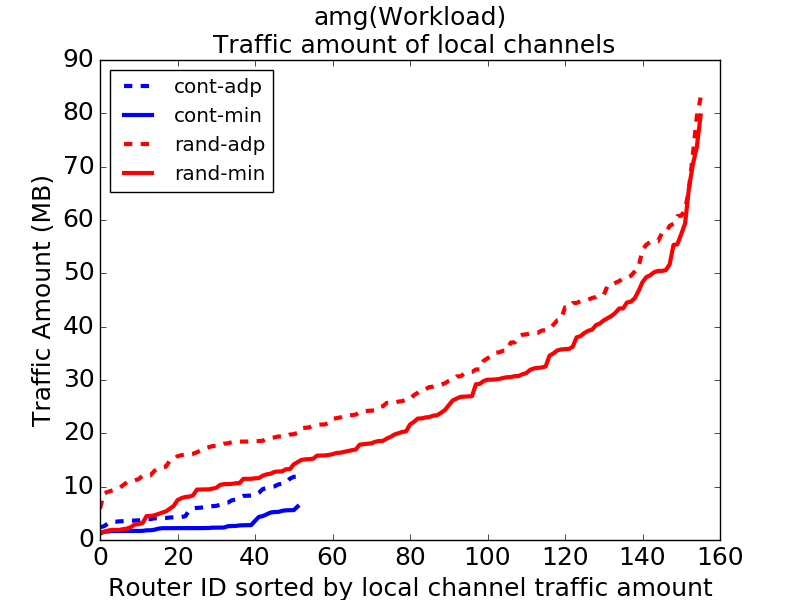
\includegraphics[height=1.8 in]{amg/lc-traffic}
        \caption{AMG Local Channel Traffic}
        \label{fig:amg-lc-traffic}
    \end{subfigure}%
    \hspace{1em}%
    \begin{subfigure}[t]{0.32\textwidth}
        \centering
        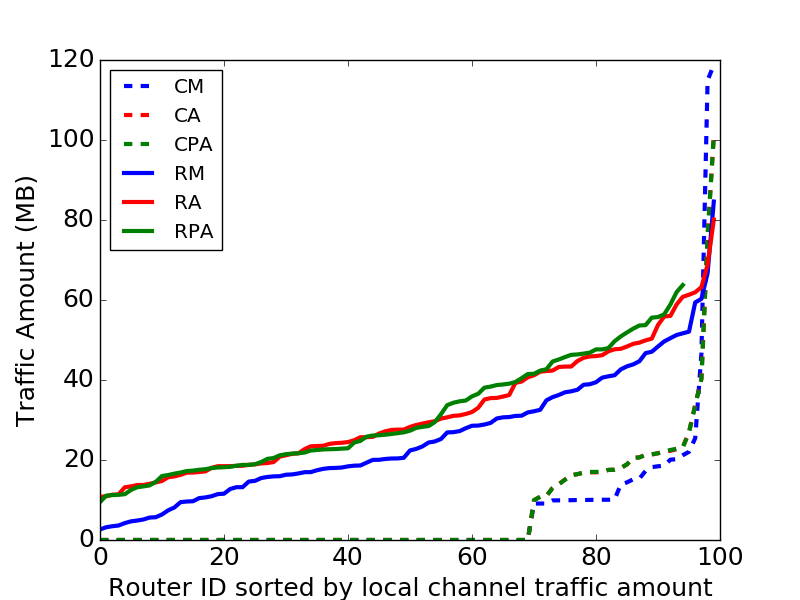
\includegraphics[height=1.8 in]{mg/lc-traffic}
        \caption{MG Local Channel Traffic}
        \label{fig:mg-lc-traffic}
    \end{subfigure}%
    \begin{subfigure}[t]{0.32\textwidth}
        \centering
        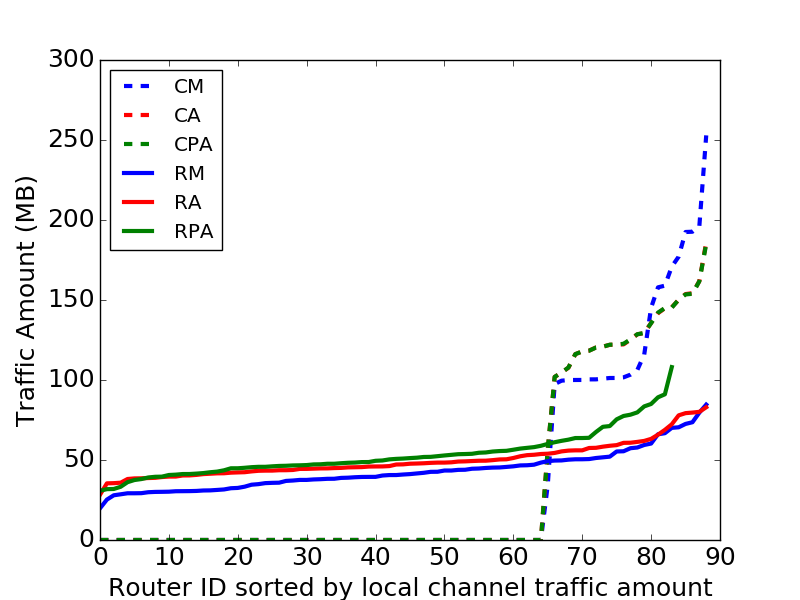
\includegraphics[height=1.8 in]{cr/lc-traffic}
        \caption{CR Local Channel Traffic}
        \label{fig:cr-lc-traffic}
    \end{subfigure}%
   \caption{Each Application Router Local Channel Traffic.  }
   \label{fig:3app-lc-traffic}
\end{figure*}


\begin{figure*}[t!]
    \centering
    \begin{subfigure}[t]{0.32\textwidth}
        \centering
        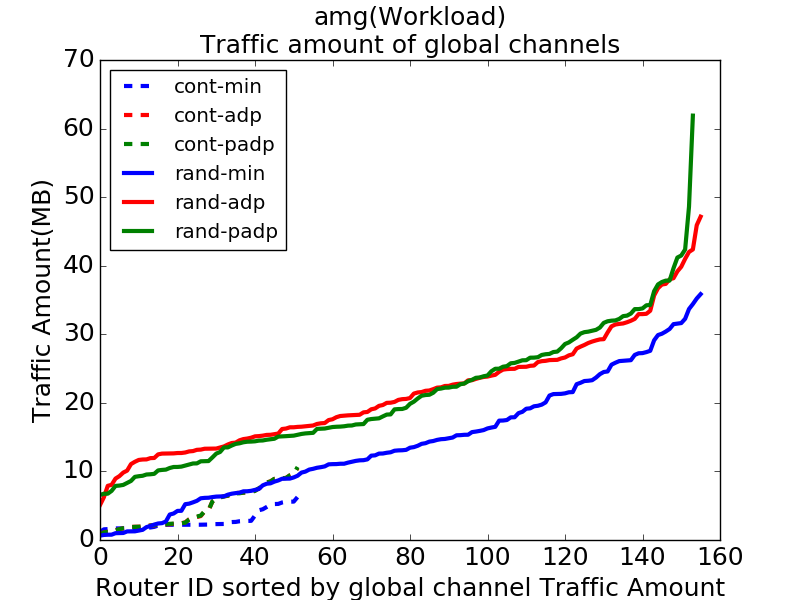
\includegraphics[height=1.8 in]{amg/gc-traffic}
        \caption{AMG Global Channel Traffic}
        \label{fig:amg-gc-traffic}
    \end{subfigure}%
    \hspace{1em}%
    \begin{subfigure}[t]{0.32\textwidth}
        \centering
        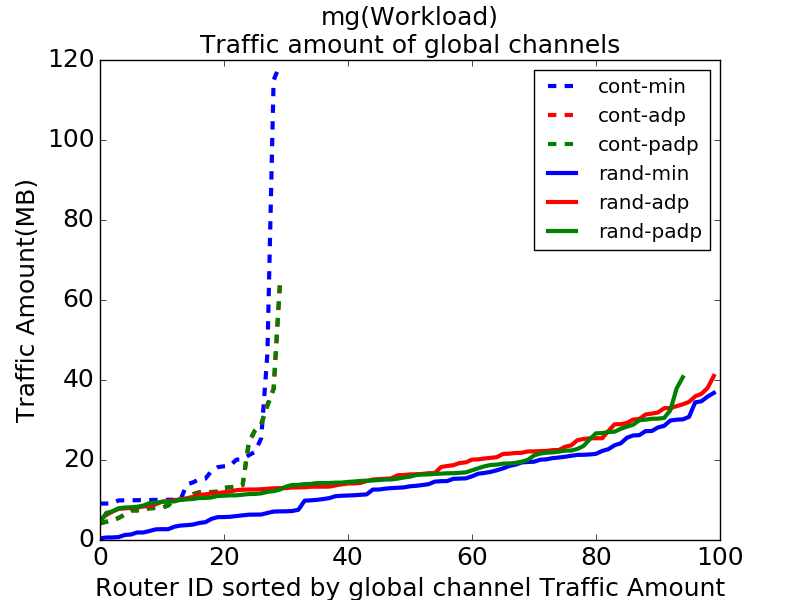
\includegraphics[height=1.8 in]{mg/gc-traffic}
        \caption{MG Global Channel Traffic}
        \label{fig:mg-gc-traffic}
    \end{subfigure}%
    \begin{subfigure}[t]{0.32\textwidth}
        \centering
        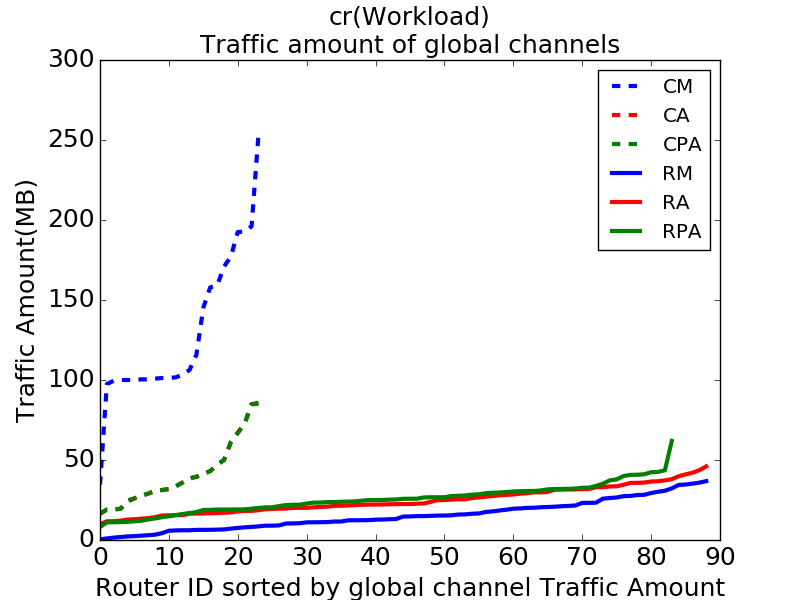
\includegraphics[height=1.8 in]{cr/gc-traffic}
        \caption{CR Global Channel Traffic}
        \label{fig:cr-gc-traffic}
    \end{subfigure}%
   \caption{Each Application Router Global Channel Traffic.}
   \label{fig:3app-gl-traffic}
\end{figure*}


Why AMG is the only victim in the workload? The reason for CrystalRouter and MultiGrid get improvement in the sacrifice of AMG's performance is that AMG is the lest communication-intensive application in the workload. As shown in Figure \ref{fig:3app-data-amount}, AMG has the least amount of data transfer between its ranks. 

\begin{figure*}[t!]
  \centering
  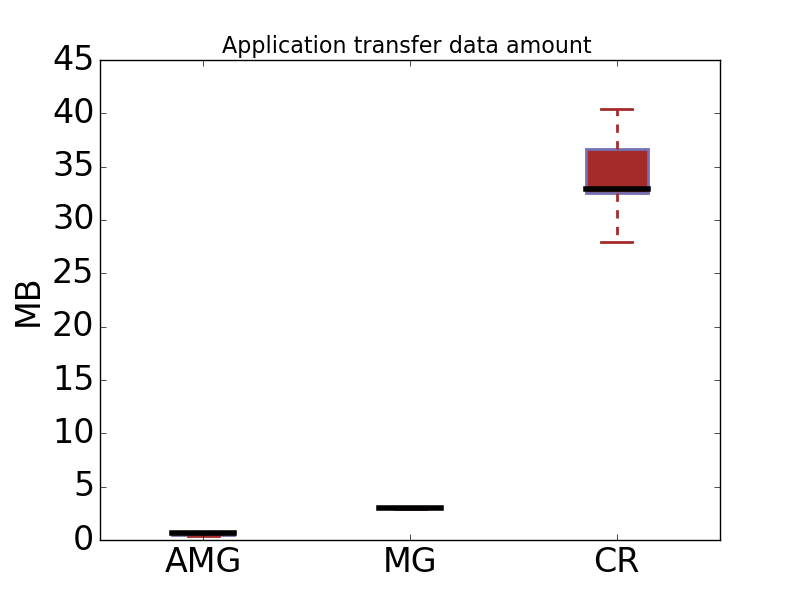
\includegraphics[height=2.2in]{data_amount}
  \caption{Applications Data Transfer Amount. AMG has the least amount of data transfer, compared with CR and MG.}
  \label{fig:3app-data-amount}
\end{figure*}

Apparently, random placement and adaptive routing is quite efficient for orchestrate the traffic load in the network. Random placement and adaptive routing can uniformly distribute the workload traffic all over the network, make the load-balanced and avoid hot-spots. However, application like AMG will be impaired in this orchestration. The routers through which the less communication-intensive application traffic used to route, now have more traffic go through them. These extra traffic are from other communication-intensive applications. Beneath the facade of harmony, less communication-intensive application are ``bullied" by their communication-intensive peers in the workload. 

We have tried three different congestion sensing schemes that used in adaptive routing\cite{dally-dragonfly}, although there are some variations of the experiments, none of the congestion sensing scheme can prevent the ``bully" from happening. 

\subsection{Analysis of Synthetic Workloads}

To validate our assumption, we generate synthetic application, sAMG, which are same the with AMG's original traces in every aspect expect that the data transfer amount 100x greater than AMG. We run the new workload that consists of sAMG, MG and CR on the same dragonfly network with the same placement and routing configurations. As shown in Figure \ref{fig:syn-3app-data-amount}, sAMG become the most communication-intensive application in the new workload. 

\begin{figure*}[t!]
  \centering
  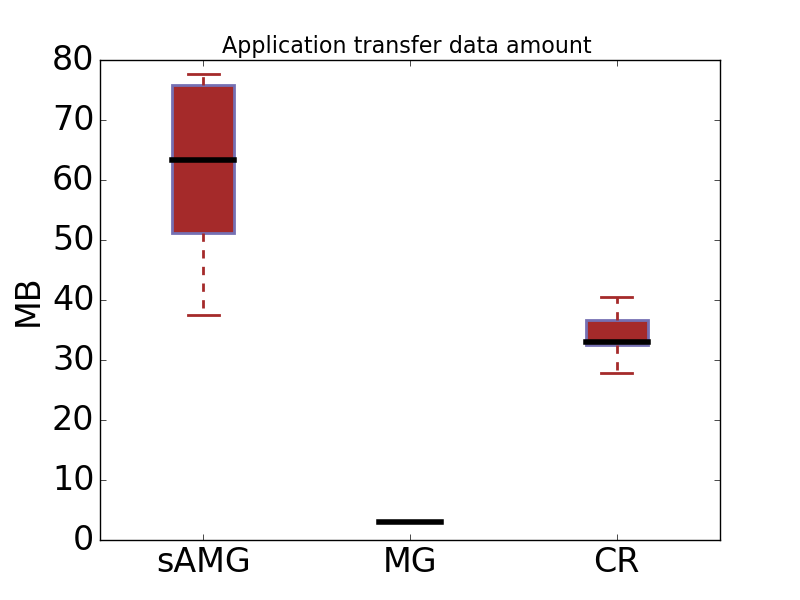
\includegraphics[height=2.2in]{syn-wkld/data_amount}
  \caption{Applications Data Transfer Amount. sAMG has the most amount of data transfer, compared with CR and MG.}
  \label{fig:syn-3app-data-amount}
\end{figure*}

The communication time of each application shown in Figure \ref{fig:syn-apps-commtime}. The ``bully" become the ``bullyee". The less communication-intensive application, CrystalRouter and MultiGrid, suffer prolonged communication time when running concurrently with sAMG with random placement and adaptive routing configuration. The routers that belongs to MultiGrid  and now CrystalRouter has extra traffic go through them, shown in Figure  \ref{fig:syn-mg-lc-traffic} \ref{fig:syn-mg-gc-traffic} and Figure \ref{fig:syn-cr-lc-traffic} \ref{fig:syn-cr-gc-traffic}. The extra traffic come from sAMG, that been redirected by adaptive routing. \textbf{More explanation about contiguous placement and minimal routing}.

\begin{figure*}[t!]
    \centering
    \begin{subfigure}[t]{0.32\textwidth}
        \centering
        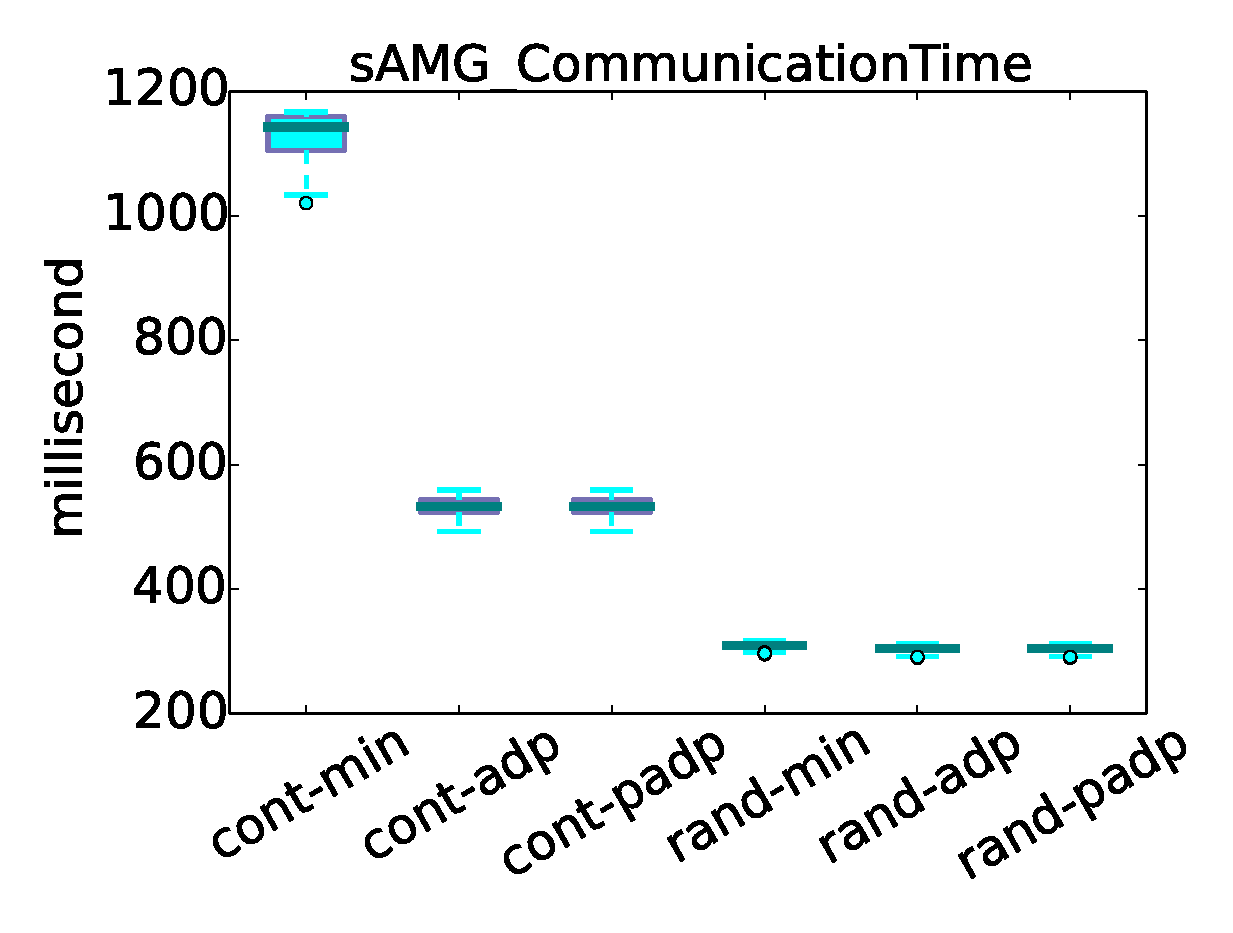
\includegraphics[height=1.5 in]{syn-wkld/amg10/commtime}
        \caption{sAMG Communication Time}
        \label{fig:samg-commtime}
    \end{subfigure}%
    \hspace{1em}%
    \begin{subfigure}[t]{0.32\textwidth}
        \centering
        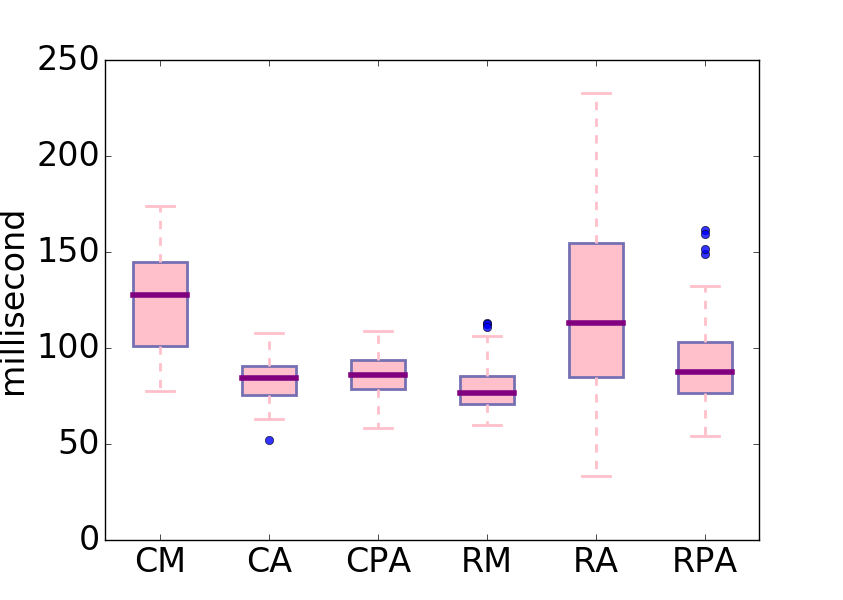
\includegraphics[height=1.5 in]{syn-wkld/mg/commtime}
        \caption{MG Communication Time}
        \label{fig:syn-mg-commtime}
    \end{subfigure}%
    \begin{subfigure}[t]{0.32\textwidth}
        \centering
        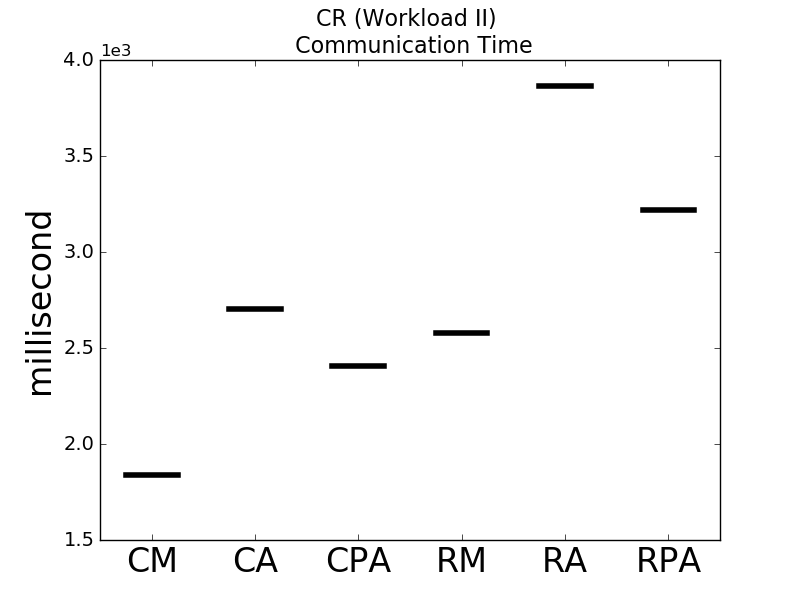
\includegraphics[height=1.5 in]{syn-wkld/cr/commtime}
        \caption{CR Communication Time}
        \label{fig:syn-cr-commtime}
    \end{subfigure}%
   \caption{Application communication time. Three applications running concurrently on dragonfly network with different placement and routing configurations. Random placement and adaptive routing can improves AMG's communication time. MG and CR communication time are prolonged with random placement and adaptive routing.}
   \label{fig:syn-apps-commtime}
\end{figure*}


\begin{figure*}[t!]
    \centering
    \begin{subfigure}[t]{0.32\textwidth}
        \centering
        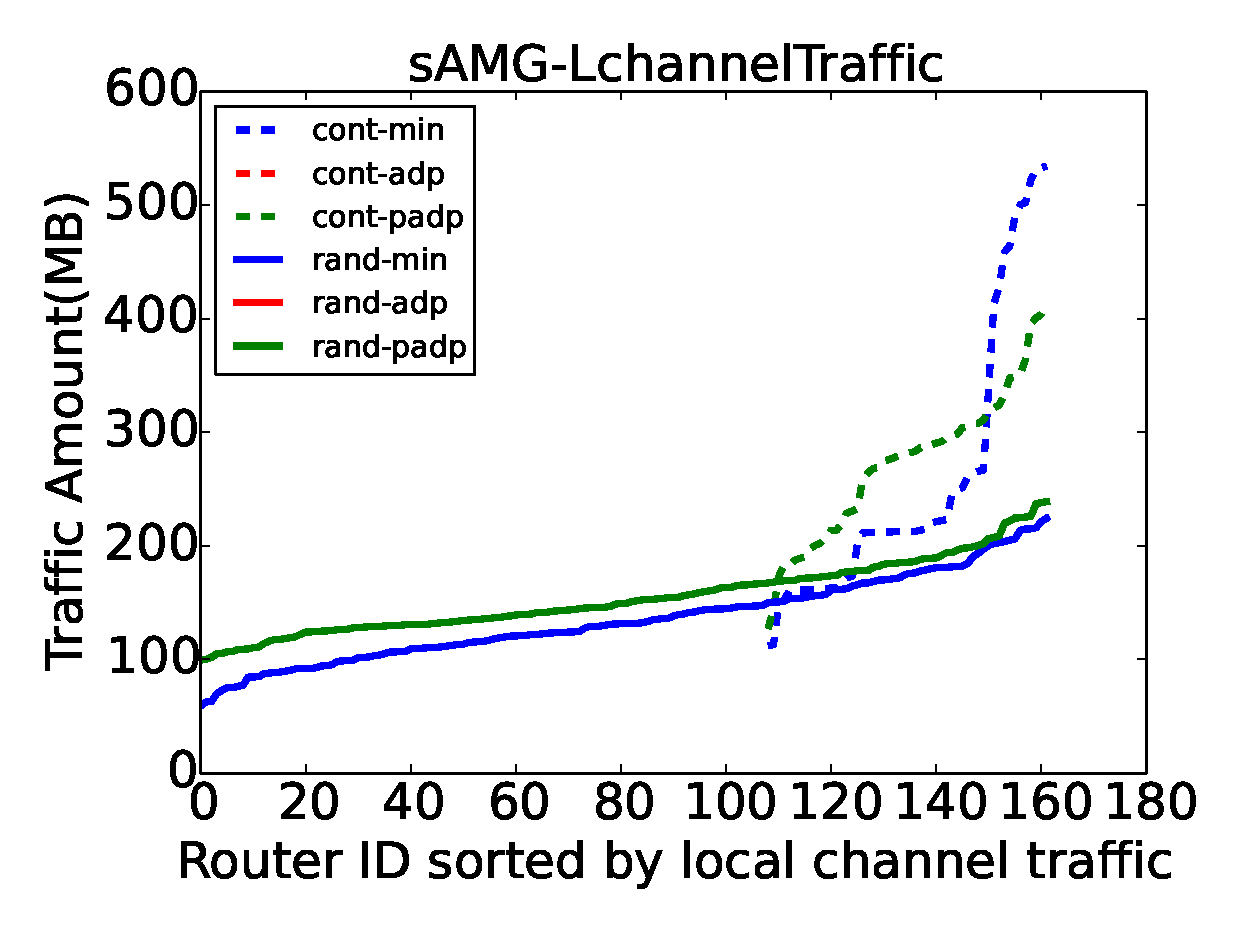
\includegraphics[height=1.5 in]{syn-wkld/amg10/lc-traffic}
        \caption{AMG Local Channel Traffic}
        \label{fig:samg-lc-traffic}
    \end{subfigure}%
    \hspace{1em}%
    \begin{subfigure}[t]{0.32\textwidth}
        \centering
        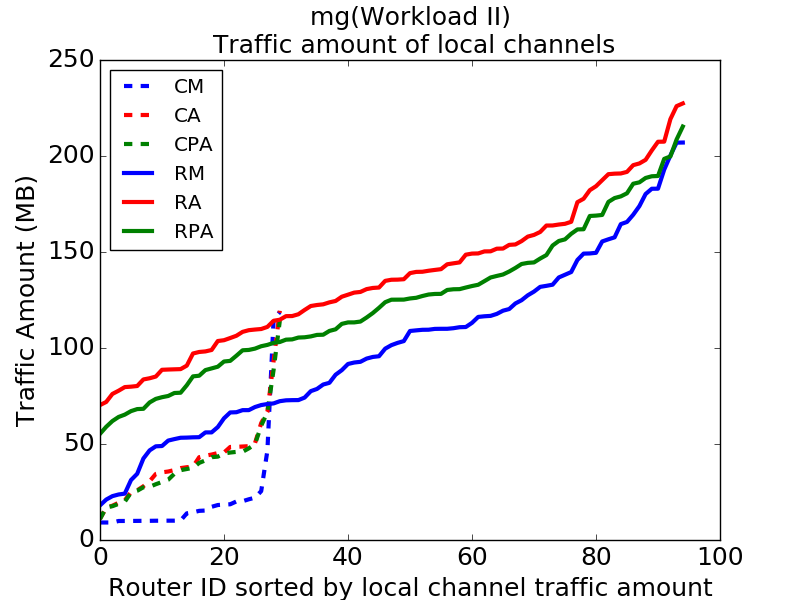
\includegraphics[height=1.5 in]{syn-wkld/mg/lc-traffic}
        \caption{MG Local Channel Traffic}
        \label{fig:syn-mg-lc-traffic}
    \end{subfigure}%
    \begin{subfigure}[t]{0.32\textwidth}
        \centering
        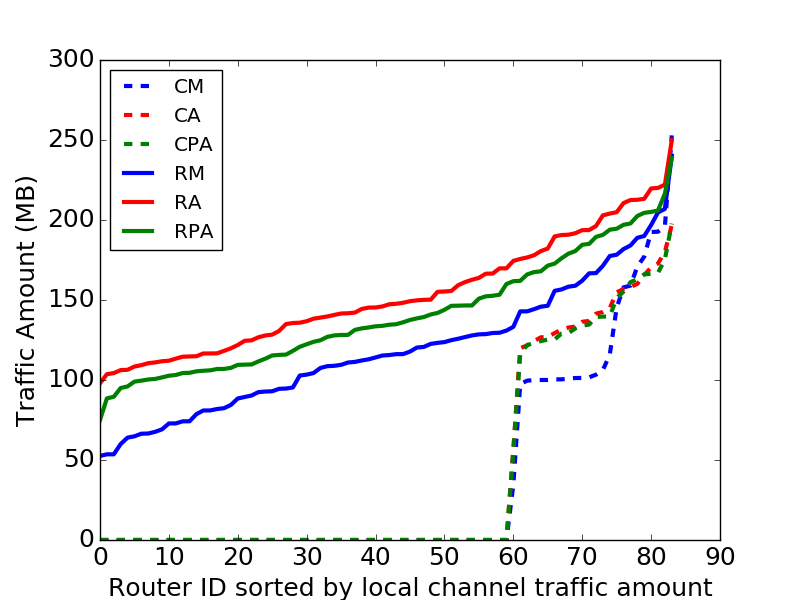
\includegraphics[height=1.5 in]{syn-wkld/cr/lc-traffic}
        \caption{CR Local Channel Traffic}
        \label{fig:syn-cr-lc-traffic}
    \end{subfigure}%
   \caption{Each Application Router Local Channel Traffic.  }
   \label{fig:syn-3app-lc-traffic}
\end{figure*}


\begin{figure*}[t!]
    \centering
    \begin{subfigure}[t]{0.32\textwidth}
        \centering
        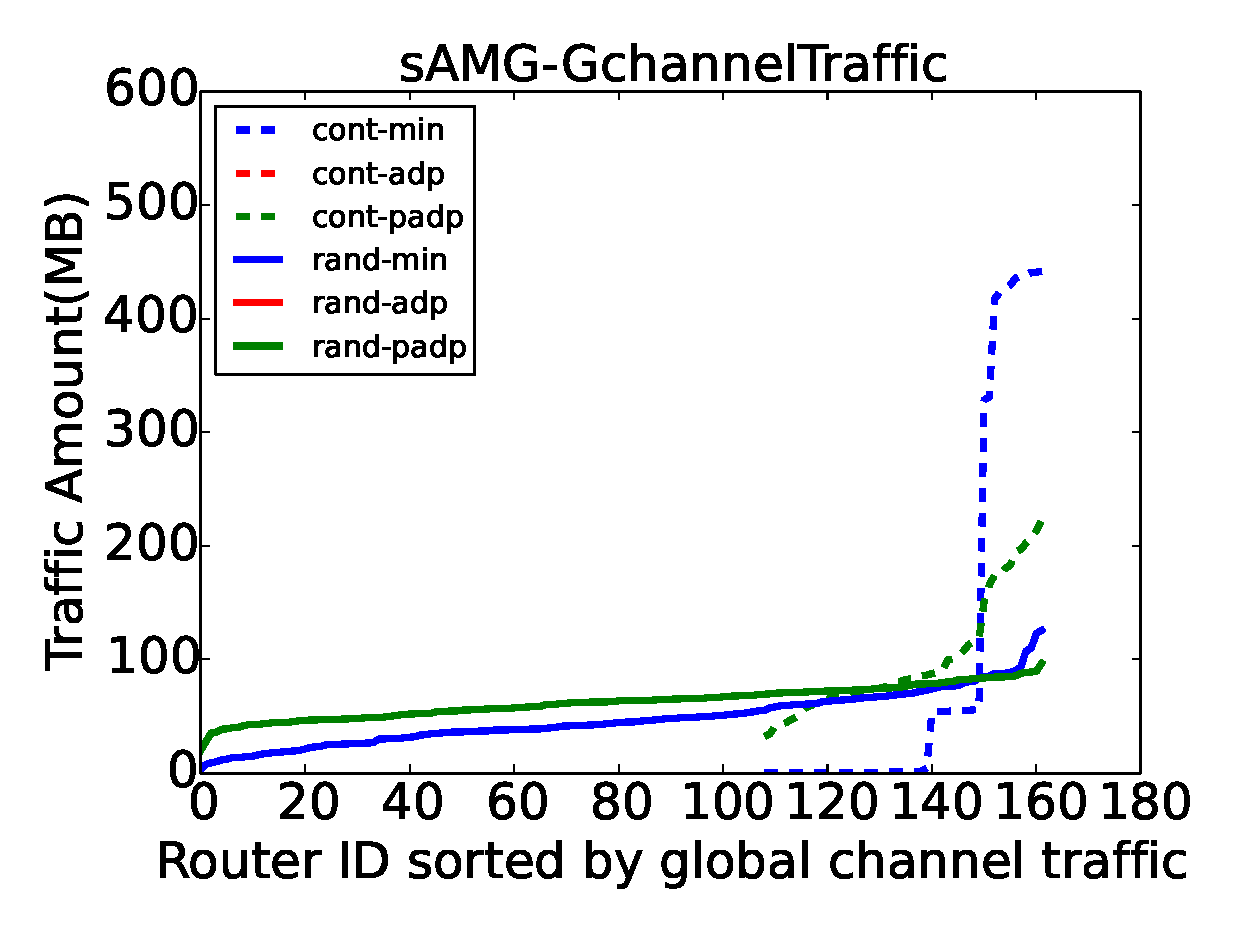
\includegraphics[height=1.5 in]{syn-wkld/amg10/gc-traffic}
        \caption{AMG Global Channel Traffic}
        \label{fig:samg-gc-traffic}
    \end{subfigure}%
    \hspace{1em}%
    \begin{subfigure}[t]{0.32\textwidth}
        \centering
        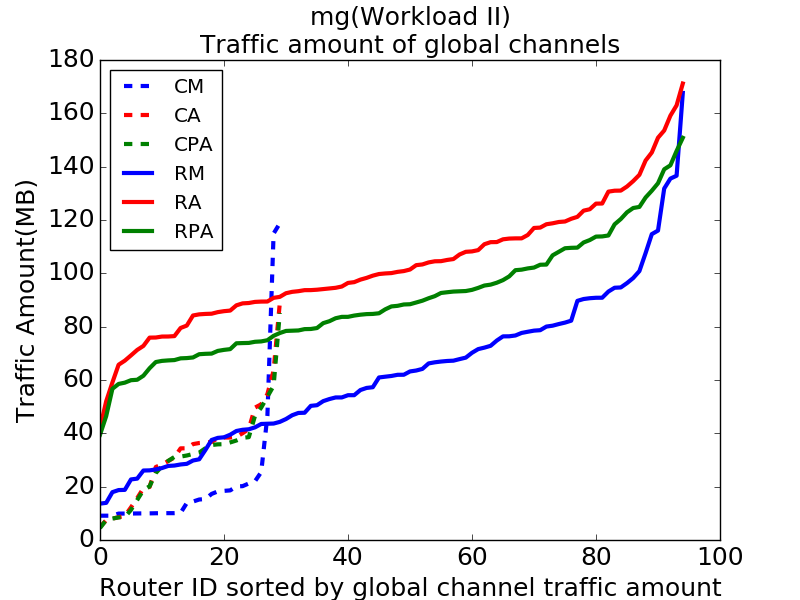
\includegraphics[height=1.5 in]{syn-wkld/mg/gc-traffic}
        \caption{MG Global Channel Traffic}
        \label{fig:syn-mg-gc-traffic}
    \end{subfigure}%
    \begin{subfigure}[t]{0.32\textwidth}
        \centering
        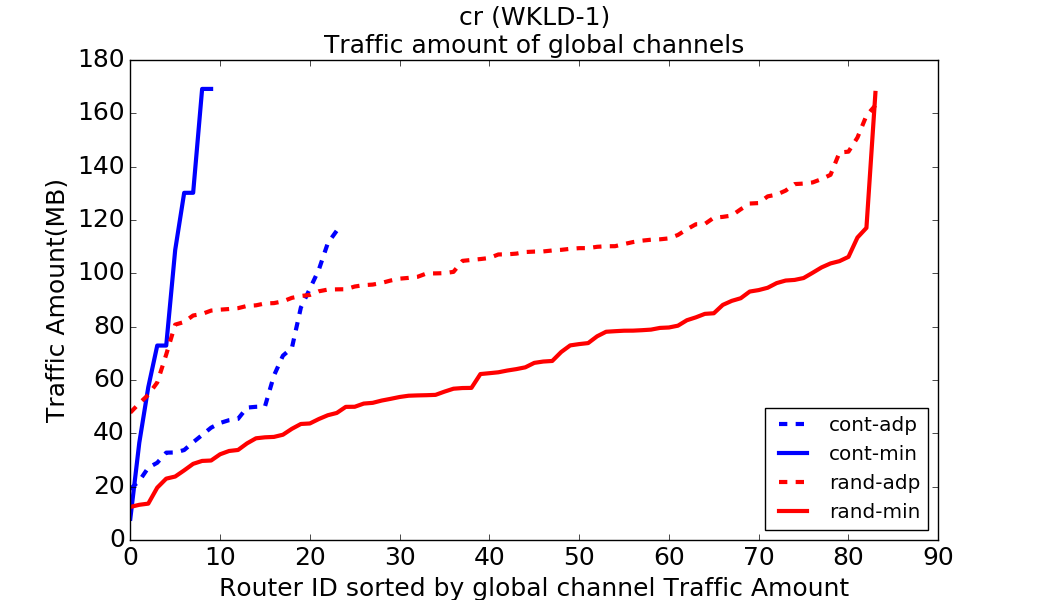
\includegraphics[height=1.5 in]{syn-wkld/cr/gc-traffic}
        \caption{CR Global Channel Traffic}
        \label{fig:syn-cr-gc-traffic}
    \end{subfigure}%
   \caption{Each Application Router Global Channel Traffic.}
   \label{fig:syn-3app-gc-traffic}
\end{figure*}


\textbf{We can add another set of synthetic workload, in which three applications have similar data transfer amount, if necessary. }

Based on the results we got from both real application traces and synthetic workload, we can make the following observations:

\begin{itemize}
    \item Random placement and adaptive routing can uniformly distribute workload traffic over the network, make the whole network load-balanced and hot-spot free. 
    \item Random placement and adaptive routing can not guarantee QoS for each application in the workload. In order to reach load-balanced and hot-spot free, the traffic from congested routers will be redirected to other less busy routers. This will indulge the ``bully" that communication-intensive applications impose to their less intensive peers. 
    \item Contiguous placement and minimal routing guarantee a consistent performance of each application. Although, contiguous placement and minimal routing usually results in local congestion and hot-spot, it can reduce the interference between concurrently running applications, thus prevent less communication-intensive application from being ``bully" by its intensive peers.
\end{itemize}


According to our findings, we believe choosing the ideal placement and routing strategies for workload running on dragonfly network should be based on application's communication intensity. The less intensive applications should avoid sharing network resource with other applications, reduce the possible interference. Contiguous placement and adaptive routing can guarantee the QoS for the less intensive applications, thus prevent the ``bully" from happening. 

The communication-intensive applications tend to cause local congestion. It is preferable to enable communication-intensive applications to have extra network resource by sharing with other applications.  Random placement and adaptive routing can alleviate the local congestion by redirecting traffic to other less busy routers in the network. 

So the ideal placement and routing strategies for workload running on dragonfly network should be like this. The communication-intensive applications should be randomly allocated over the system and adaptive routing should be used by these applications to alleviate the local congestion. On the other hand, less intensive application should get contiguous allocation, minimal routing should be used by these applications to avoid network sharing and reduce interference. 
 


\section{Related Work}
\label{sec:related work}

The impact of job placement to both system and application always catch researchers appetite \cite{dskinner} \cite{abhinav-sc13} \cite{jose-ipdps15}. Skinner et al.\cite{dskinner} identified that network congestion could cause significant performance variability. Bhatele et al. \cite{abhinav-sc13} studied the performance variability of a specific application, p3FD, running on different production system. They noticed that the application performance would keep consistent when it got compact allocation and exclusive network resource. Jokanovic et al.\cite{jose-ipdps15} study the impact of job placement to the workload and claimed that the key to reduce performance variability is to avoid network sharing. 

Recently, several researchers have investigated the job placement and routing schemes on dragonfly network. Bogdan et al \cite{hoefler-hpdc14} proposed novel solution for mapping tasks of application that conforms to Nearest Neighbor communication pattern on dragonfly network. Jain et al. \cite{jain-sc14} conducted a comprehensive analysis of various job placement and routing scheme with regard to network link throughput on dragonfly network. Their work is based on an analytical model and synthetic workload. Bhatele et al.\cite{bhatele-sc11} used simulation to study the performance of synthetic workload under the different task mapping and routing schemes on two-level direct networks.


Our work different from the previous works in the following ways. First, instead of using synthetic workload that generated based on predefined communication patterns, our simulation is driven real application traces collected from production system. Second, not only we care about the workload performance, but also we pay attention to each individual application in the workload. We found that although random placement and adaptive routing can improve the workload performance, some specific application in the workload may suffer performance degradation. Third, with the sophisticated simulation tool CODES, we can get not only applications communication information, but also we have the insight about the network status when application is running. The traffic and busy time of router's each link are valuable information for detailed analysis.


% An example of a floating figure using the graphicx package.
% Note that \label must occur AFTER (or within) \caption.
% For figures, \caption should occur after the \includegraphics.
% Note that IEEEtran v1.7 and later has special internal code that
% is designed to preserve the operation of \label within \caption
% even when the captionsoff option is in effect. However, because
% of issues like this, it may be the safest practice to put all your
% \label just after \caption rather than within \caption{}.
%
% Reminder: the "draftcls" or "draftclsnofoot", not "draft", class
% option should be used if it is desired that the figures are to be
% displayed while in draft mode.
%
%\begin{figure}[!t]
%\centering
%\includegraphics[width=2.5in]{myfigure}
% where an .eps filename suffix will be assumed under latex, 
% and a .pdf suffix will be assumed for pdflatex; or what has been declared
% via \DeclareGraphicsExtensions.
%\caption{Simulation results for the network.}
%\label{fig_sim}
%\end{figure}

% Note that the IEEE typically puts floats only at the top, even when this
% results in a large percentage of a column being occupied by floats.


% An example of a double column floating figure using two subfigures.
% (The subfig.sty package must be loaded for this to work.)
% The subfigure \label commands are set within each subfloat command,
% and the \label for the overall figure must come after \caption.
% \hfil is used as a separator to get equal spacing.
% Watch out that the combined width of all the subfigures on a 
% line do not exceed the text width or a line break will occur.
%
%\begin{figure*}[!t]
%\centering
%\subfloat[Case I]{\includegraphics[width=2.5in]{box}%
%\label{fig_first_case}}
%\hfil
%\subfloat[Case II]{\includegraphics[width=2.5in]{box}%
%\label{fig_second_case}}
%\caption{Simulation results for the network.}
%\label{fig_sim}
%\end{figure*}
%
% Note that often IEEE papers with subfigures do not employ subfigure
% captions (using the optional argument to \subfloat[]), but instead will
% reference/describe all of them (a), (b), etc., within the main caption.
% Be aware that for subfig.sty to generate the (a), (b), etc., subfigure
% labels, the optional argument to \subfloat must be present. If a
% subcaption is not desired, just leave its contents blank,
% e.g., \subfloat[].


% An example of a floating table. Note that, for IEEE style tables, the
% \caption command should come BEFORE the table and, given that table
% captions serve much like titles, are usually capitalized except for words
% such as a, an, and, as, at, but, by, for, in, nor, of, on, or, the, to
% and up, which are usually not capitalized unless they are the first or
% last word of the caption. Table text will default to \footnotesize as
% the IEEE normally uses this smaller font for tables.
% The \label must come after \caption as always.
%
%\begin{table}[!t]
%% increase table row spacing, adjust to taste
%\renewcommand{\arraystretch}{1.3}
% if using array.sty, it might be a good idea to tweak the value of
% \extrarowheight as needed to properly center the text within the cells
%\caption{An Example of a Table}
%\label{table_example}
%\centering
%% Some packages, such as MDW tools, offer better commands for making tables
%% than the plain LaTeX2e tabular which is used here.
%\begin{tabular}{|c||c|}
%\hline
%One & Two\\
%\hline
%Three & Four\\
%\hline
%\end{tabular}
%\end{table}


% Note that the IEEE does not put floats in the very first column
% - or typically anywhere on the first page for that matter. Also,
% in-text middle ("here") positioning is typically not used, but it
% is allowed and encouraged for Computer Society conferences (but
% not Computer Society journals). Most IEEE journals/conferences use
% top floats exclusively. 
% Note that, LaTeX2e, unlike IEEE journals/conferences, places
% footnotes above bottom floats. This can be corrected via the
% \fnbelowfloat command of the stfloats package.




\section{Conclusion}
The conclusion goes here.




% conference papers do not normally have an appendix



% use section* for acknowledgment
\ifCLASSOPTIONcompsoc
  % The Computer Society usually uses the plural form
  \section*{Acknowledgments}
\else
  % regular IEEE prefers the singular form
%   \section*{Acknowledgment}
\fi


The authors would like to thank...


% trigger a \newpage just before the given reference
% number - used to balance the columns on the last page
% adjust value as needed - may need to be readjusted if
% the document is modified later
%\IEEEtriggeratref{4}


\bibliographystyle{IEEEtran}
\bibliography{./reference}  


% \vspace{5\baselineskip}
% 
% \begin{framed}
% The submitted manuscript has been created by UChicago Argonne, LLC, Operator of Argonne National Laboratory ("Argonne").  Argonne, a U.S. Department of Energy Office of Science laboratory, is operated under Contract No. DE-AC02-06CH11357.  The U.S. Government retains for itself, and others acting on its behalf, a paid-up nonexclusive, irrevocable worldwide license in said article to reproduce, prepare derivative works, distribute copies to the public, and perform publicly and display publicly, by or on behalf of the Government.
% \end{framed}




% that's all folks
\end{document}


